% Type of the document
\documentclass[11pt]{beamer}

% elementary packages:
\usepackage{graphicx}
%\usepackage[latin1]{inputenc}
\usepackage[T1]{fontenc}
\usepackage[vietnamese]{babel}
%\usepackage[utf8]{vietnam} 
\usepackage{listings}
\usepackage{xcolor}
\usepackage{eso-pic}
\usepackage{mathrsfs}
\usepackage{url}
\usepackage{amssymb}
\usepackage{amsmath}
\usepackage{multirow}
\usepackage{hyperref}
\usepackage{booktabs}
\usepackage{tikz}
\usetikzlibrary{arrows.meta}
\usepackage{xcolor}
\usepackage{bm}
\newcommand*{\B}[1]{\ifmmode\bm{#1}\else\textbf{#1}\fi}



% additional packages
\usepackage{bbm}

% packages supplied with ise-beamer:
\usepackage{cooltooltips}
\usepackage{colordef}
\usepackage{beamerdefs}
\usepackage{lvblisting}

% Mathematics
\usepackage{amssymb}
\usepackage{amsmath}
\usepackage{mathrsfs}
\usepackage{amsthm,amsfonts}
\usepackage{mathtools}
\usepackage{algorithmic}
\usepackage[linesnumbered,ruled]{algorithm2e}
\usepackage{float}

% Itemize custom
\usepackage{enumitem}
\usepackage{xcolor}


\newcommand{\ra}{\rightarrow}
\newcommand{\Ra}{\Rightarrow}
\newcommand{\lra}{\longrightarrow}
\newcommand{\Lra}{\Longrightarrow}
\newcommand{\la}{\leftarrow}
\newcommand{\La}{\Leftarrow}
\newcommand{\lla}{\longleftarrow}
\newcommand{\Lla}{\Longleftarrow}
\newcommand{\Llra}{\Longleftrightarrow}
\newcommand{\map}{\longmapsto}
\newcommand{\al}{\alpha}
\newcommand{\bt}{\beta}
\newcommand{\dt}{\delta}
\newcommand{\De}{\Delta}
\newcommand{\tta}{\theta}
\newcommand{\e}{\varepsilon}
\newcommand{\vp}{\varphi}
\newcommand{\na}{\nabla}
\newcommand{\pa}{\partial}
\newcommand{\sm}{\sigma}
\newcommand{\Sm}{\Sigma}
\newcommand{\Gm}{\Gamma}
\newcommand{\gm}{\gamma}
\newcommand{\Om}{\Omega}
\newcommand{\R}{\mathbb R}
\newcommand{\Q}{\mathbb Q}
\newcommand{\N}{\mathbb N}
\newcommand{\Z}{\mathbb Z}
\newcommand{\Oo}{\mathcal O}
\newcommand{\K}{\mathcal K}
\newcommand{\G}{\mathcal G}
\newcommand{\D}{\mathcal D}
\newcommand{\X}{\mathcal X}
\newcommand{\M}{\mathcal M}
\newcommand{\T}{\mathcal T}
\newcommand{\V}{\mathcal V}
\newcommand{\W}{\mathcal W}
\newcommand{\PP}{\mathcal P}
\newcommand{\QQ}{\mathcal Q}
\newcommand{\UU}{\mathcal U}
\newcommand{\LL}{\mathcal L}
\newcommand{\cbe}{\scriptsize}
\newcommand{\On}{\widetilde{\mathcal{O}}}
\newcommand{\Mn}{\widetilde{M}}
\newcommand{\wt}[1]{\widetilde #1}
\newcommand{\sumh}{\overline{\sum}}
\newcommand{\cho}[2]{\ensuremath{#1\choose#2}}
\newcommand{\ve}[1]{{\bf #1}}

\DeclareMathOperator{\Div}{div}
\DeclareMathOperator{\Vol}{Vol}
\DeclareMathOperator*{\argmin}{argmin}
\DeclarePairedDelimiter{\norm}{\lVert}{\rVert}
\DeclarePairedDelimiter{\abs}{\lvert}{\rvert}

\newtheorem{Not}{Notation}
\newtheorem{Hypo}{Hypothesis}
\newtheorem{Theo}{Theorem}%[section]
\newtheorem{Prop}{Proposition}%[section]
\newtheorem{Coro}{Corollary}%[section]
\newtheorem{Algo}{Algorithm}

\theoremstyle{definition}
\newtheorem{Defi}{Definition}%[section]

\theoremstyle{plain}
\newtheorem{Lem}{Lemma}%[section]
\theoremstyle{plain}
\newtheorem{Assu}{Assumption}
\usepackage[backend=biber,style=numeric, citestyle=ieee]{biblatex}
\addbibresource{sample.bib}
\theoremstyle{remark}
\newtheorem*{Rem}{Remark}
%\usepackage{caption}
\usepackage{subcaption}


% Định nghĩa màu tím với mã màu HEX
\definecolor{myPurple}{HTML}{3333B2}
% Định dạng cho toàn bộ itemize
\setlist[itemize]{
	label=\textcolor{myPurple}{$\bullet$},
	left=0.6cm
}
\newcommand{\myitem}{\item[\tikz{\draw[ball color=myPurple,shade] (0,0) circle (0.17em);}]}



% Change the pictures here:
% logobig and logosmall are the internal names for the pictures: do not modify them. 
% Pictures must be supplied as JPEG, PNG or, to be preferred, PDF
\pgfdeclareimage[height=3cm]{logobig}{Figures/logoptit}
% Supply the correct logo for your class and change the file name to "logo". The logo will appear in the lower
% right corner:
\pgfdeclareimage[height=1cm]{logosmall}{Figures/logoptit}

% Title page outline:
% use this number to modify the scaling of the headline on title page
\renewcommand{\titlescale}{1.0}
% the title page has two columns, the following two values determine the percentage each one should get
\renewcommand{\titlescale}{1.0}
\renewcommand{\leftcol}{0.6}

% smaller font for selected slides
\newcommand\Fontvi{\fontsize{10}{7.2}\selectfont}
\newcommand\Fontsm{\fontsize{8}{7.2}\selectfont}
%\usepackage{caption}

% Define the title. Don't forget to insert an abbreviation instead 
% of "title for footer". It will appear in the lower left corner:
\title[ \footnotesize  \textcolor{red}{\bf Đồ án tốt nghiệp} -- \textcolor{blue}{Trần Xuân Độ - Đặng Thị Thoa}]{\Large  \bf BẢO VỆ ĐỒ ÁN}
% Define the authors:
\authora{\bfseries \textcolor{blue}{\Large Chủ đề: Bao lồi và ứng dụng trong việc phát hiện hiện định hướng và đóng gói đối tượng}\vspace{20pt}} % a-c

\authorb{ Giảng viên hướng dẫn: Nguyễn Kiều Linh \\ Sinh viên thực hiện:\\ \textcolor{blue}{1. Trần Xuân Độ - B19DCCN}\\ \textcolor{blue}{2. Đặng Thị Thoa - B19DCCN676}
}
%\def\linka{}



% Define any internet addresses, if you want to display them on the title page:
%\def\linka{http://www.ptit.edu.vn}
\def\linkb{}
\def\linkc{}
% Define the institute:
\institute{\bf  Hà Nội, năm 2023\\}

% Comment the following command, if you don't want, that the pdf file starts in full screen mode:
%\hypersetup{pdfpagemode=FullScreen}

%%%%
% Main document
%%%%
\setbeamertemplate{section in toc}[square]
\setbeamertemplate{subsection in toc}[ball unnumbered]
\AtBeginSection[]
{
	\begin{frame}
	\frametitle{Nội dung chính}
	\tableofcontents[currentsection]
\end{frame}
}% mỗi đầu section thì thêm 1 frame mục lục làm nổi bật section đó%
\AtBeginSubsection[]
{
\begin{frame}
\frametitle{Nội dung chính}
\tableofcontents[currentsection,currentsubsection]
\end{frame}
}

\begin{document}
\begin{frame}{\begin{center}
			Chào mừng các thầy cô đến với buổi bảo vệ đồ án!
	\end{center}}
	\begin{center}
	{\large	\textbf{Đề tài}: Bao lồi xấp xỉ - Bao lồi trực giao trong định hướng và phát hiện đối tượng \\
		có hướng.\\}
	\end{center}
	
	\textbf{Giảng viên hướng dẫn:} TS.Nguyễn Kiều Linh.\\
	
	\textbf{Sinh viên thực hiện}: Trần Xuân Độ - Đặng Thị Thoa.\\
	
	\textbf{Năm bảo vệ:} 2023
	
	
\end{frame}

\begin{frame}{Giới thiệu nội dung}
	1. Giới thiệu bài toán.
	\begin{itemize}
		\myitem Đặt vấn đề.
		\myitem Phương pháp thích ứng bao lồi (Convex-hull feature adaptation - CFA).
	 \end{itemize}
	2. Thuật toán bao lồi xấp xỉ.
	\begin{itemize}
		\myitem Outer convex approximation.
		\myitem Inner convex approximation. 
	\end{itemize}
	3. Thuật toán bao lồi trực giao. 
	\begin{itemize}
		\myitem Các khái niệm. 
		\myitem Thuật toán tìm bao lồi Quickhull.
	\end{itemize}
	4. Thực nghiệm và kết quả.
	\begin{itemize}
		\myitem Các bước triển khai.
		\myitem Một vài kết quả số.
	\end{itemize}
	
\end{frame}
%\Fontvi 
% Draw title page

%\begin{frame}{Lời cảm ơn}
	
%	Em xin chân thành cảm ơn TS. Nguyễn Kiều Linh và tất cả quý thầy cô tại Học viện Công nghệ Bưu chính Viễn thông. Nhờ sự hướng dẫn và hỗ trợ nhiệt tình của TS. Nguyễn Kiều Linh, em đã có cơ hội thực hiện đồ án tốt nghiệp một cách thành công. Cảm ơn cô đã luôn nhiệt tình hỏi thăm và đóng góp ý kiến quan trọng vào quá trình xây dựng sản phẩm.
	
%	Đồng thời, em cũng muốn bày tỏ lòng biết ơn đến Học viện và tất cả các quý thầy cô đã tạo điều kiện và môi trường giáo dục tích cực, giúp em có cơ hội học tập và phát triển kiến thức. Những kiến thức này không chỉ hỗ trợ em trong việc hoàn thành đồ án mà còn là nền tảng cho tương lai nghề nghiệp của em. Cảm ơn sự tận tâm và nhiệt huyết trong việc giảng dạy của quý thầy cô.
%\end{frame}

\section{Giới thiệu bài toán}

\subsection{Đặt vấn đề}
\begin{frame}{Đặt vấn đề}
	Việc định vị và phát hiện đối tượng dày đặc vẫn còn nhiều thách thức: đặc trưng răng cưa (feature aliasing)
	\begin{itemize}
		\item Hiện tượng các bounding-box hình chữ nhật giao nhau ở các góc
		\item Trường tiếp nhận không tách rời nhau
		\item Phân biệt đối tượng trở nên khó khăn
	\end{itemize}
%Trong bài toán phát hiện đối tượng, việc định vị và phát hiện đối tượng dày đặc vẫn còn là một vấn đề thách thức do vấn đề đặc trưng răng cưa (feature aliasing), tức là các pi. Có các giải pháp đã được sử dụng: làm giàu các đặc trưng (enhance features) và sử dụng anchors. Nhược điểm của các phương pháp này: làm cho cấu trúc mạng trở nên phức tạp hơn, tăng thời gian huấn luyện (training) và suy luận (inference). Một phương pháp khác đó là sử dụng biến đổi
%RoI, nhưng phương pháp này không thích ứng tốt với các đối tượng có hướng bất kỳ, đặc biệt đối với các đối tượng xuất hiện dày đặc trong hình ảnh.
% Để giải quyết vẫn đề đó, một phương pháp đã được đưa ra: phương pháp thích ứng bao lồi (convex-hull feature adaptation-CFA).
\end{frame}

\begin{frame}{Minh họa vấn đề}
	\begin{columns}[c] % Căn giữa các cột
		\column{.5\textwidth} % Cột 1 chiếm 50% của khung
		\begin{figure}
			\centering
			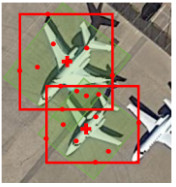
\includegraphics[width=3cm]{reppoint_bouding_box.jpg}
			\caption{RepPoint Bounding Box.}
		\end{figure}
		
		\column{.5\textwidth} % Cột 2 chiếm 50% của khung
		\begin{figure}
			\centering
			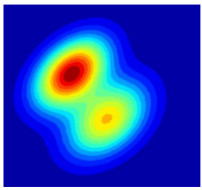
\includegraphics[width=3cm]{reception_field_w_aliasing.jpg}
			\caption{Reception Field with aliasing.}
		\end{figure}
	\end{columns}
\end{frame}

\begin{frame} {Giải quyết vấn đề}
	Để giải quyết vấn đề feature aliasing, sử dụng phương pháp thích ứng bao lồi - CFA:
	\begin{itemize}
		\item Sử dụng bao lồi thay cho hình chữ nhật làm bouding box.
		\item Hạn chế sự giao nhau giữa các bounding box.
		\item Giúp cho việc phát hiện đối tượng trở nên hiệu quả hơn
	\end{itemize}
	
	
\end{frame}
\begin{frame}{Hình ảnh minh họa}
	\begin{columns}[c] % Căn giữa các cột
		\column{.5\textwidth} % Cột 1 chiếm 50% của khung
		\begin{figure}
			\centering
			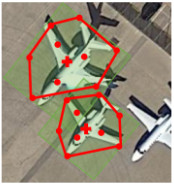
\includegraphics[width=3cm]{ConvexHull_Bouding_Box.jpg}
			\caption{ConvexHull Bounding Box.}
		\end{figure}
		
		\column{.5\textwidth} % Cột 2 chiếm 50% của khung
		\begin{figure}
			\centering
			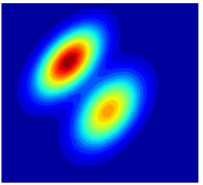
\includegraphics[width=3cm]{reception_field_wo_aliasing.jpg}
			\caption{Reception Field without aliasing.}
		\end{figure}
	\end{columns}
\end{frame}
\subsection{Phương pháp thích ứng bao lồi (convex-hull feature adaptation-CFA)}

\begin{frame}{Phương pháp thích ứng bao lồi (convex-hull feature adaptation-CFA)}

CFA được thực hiện dựa trên phương pháp biểu diễn bao lồi, định nghĩa một tập các điểm đặc trưng, giới hạn phạm vi của đối tượng mục tiêu sử dụng chỉ số CIoU.\\
CFA đạt được sự phân bổ đặc trưng tối ưu nhờ vào việc xây dựng tập bao lồi và phân
chia linh hoạt các bao lồi thành các bao lồi âm và bao lồi dương.\\



\end{frame}
\begin{frame}{Minh họa bộ phát hiện CFA}
	\begin{figure}[htp]
		\begin{center}
			\includegraphics[width=10cm]{./Hình 1.jpg}
			\caption{Sơ đồ luồng của bộ dò CFA được đề xuất.}
			\label{fig_dhandang1 }
		\end{center}
	\end{figure}
\end{frame}
\begin{frame}{Xây dựng tập bao lồi}
	
	Phương pháp CFA đã đề xuất biểu diễn phạm
	vi của đối tượng bằng bao lồi. Mỗi bao lồi là một tập hợp các điểm thoả mãn
	công thức:
	\begin{align} \label{ptdd}
		C_i = \{(x_i^k, y_i^k )\}_i^{k=1,2,...,K}
	\end{align}
	
	Trong đó $k$ là chỉ số của các điểm đặc trưng và $\mathbb{K}$ = 9 là số điểm đặc trưng của lồi. 
	
	
\end{frame}
\begin{frame}{2 giai đoạn thực hiện:}
	\begin{itemize}
		\item[-]  Giai đoạn 1: tạo tập bao lồi và ước lượng sơ bộ bố cục của bao lồi.
		
		\item[-] Giai đoạn 2: chỉnh sửa bao lồi sao cho phù hợp với các đối tượng phân bổ dày đặc.
		
	\end{itemize}
\end{frame}


\begin{frame}{Giai đoạn 1}
	Việc huấn luyện có thể xem như là quá trình dự đoán độ lệch (offset), trong
	khi hệ số CIoU cần được tối đa hoá để đạt được so khớp tối ưu nhất.
	\begin{align} \label{ptdd}
		\widehat C_l (\theta) \gets \{(x_i^k + \Delta x_i^k, y_i^k + \Delta y_i^k )\}_i^{k=1,2,...,K}
	\end{align}
	trong đó $\theta$ là các tham số của mạng. Việc dự đoán offset sẽ thực
	hiện theo công thức trên.
\end{frame}

\begin{frame}{Tích chập biến dạng}
Tích chập biến dạng (Deformable convolution - DCN) [2] là dạng tích chập
mà vị trí thực hiện tích chập bị biến dạng, không giống tích chập truyền thống
là dạng lưới NxN. Ưu điểm của phương pháp này giúp trích xuất các đặc trưng
mong muốn được chính xác hơn, lấy mẫu được ở những vị trí đa dạng hơn 

\begin{figure}[ht!]
	\begin{center}
		\includegraphics[width=8cm]{./Hình 6.jpg}
		\caption{Sơ đồ phép chiếu để xác định kết quả sau phép tích chập.}
		\label{fig_dhandang6 }
	\end{center}
\end{figure}

\end{frame}


\begin{frame}{Thuật toán tìm bao lồi}
Chia làm 2 hướng xử lý:
\begin{itemize}
	\item[-] Thuật toán tìm bao lồi xấp xỉ - Outer Convex Approximation.
	
	\item[-]  Thuật toán tìm bao lồi trực giao - Orthogonal Quick Hull.
	
\end{itemize}	
\end{frame}

\begin{frame}{Định nghĩa công thức Convex Intersection over Union (CIoU)}
Dựa trên mỗi dự đoán bao lồi, có thể tính toán độ chênh lệch về vị trí và phân loại cho mỗi đối tượng. Giá trị CIoU giữa đối tượng thứ $i$ dự đoán convex-hull $C_i (\theta)$ và hộp thực $\mathcal{B}_j$ của đối tượng thứ $j$ được tính toán như sau:
\begin{align} \label{ptdd}
	CIoU_{(C_i (\theta), B_j)} (\theta) = \frac{|C_i(\theta) \cap B_j|}{|C_i(\theta) \cup B_j|} - \frac{|R_j \setminus (C_i(\theta) \cup B_j)|}{|R_j|}
\end{align}
- $R_j$: đa giác nhỏ nhất bao quanh cả hai $C_i(\theta)$ và $B_j$.\\
CIoU không chỉ có thể đại diện cho phần chống lấn không gian mà còn là hàm liên tục và có khả năng đạo hàm.
\end{frame}


\begin{frame}{Convex-Hull Localization Loss}
Chia làm hai hàm loss: Localization Loss và Classification Loss.\\
 Có thể sử dụng chỉ số CIoU để làm hàm loss do tính chất tương tự 1 hàm loss.\\
 Hàm loss localization được định nghĩa như sau:
\begin{align} \label{ptdd0}
	\mathcal{L}_i^{loc} (\theta) = 1 - CIoU(C_i(\theta), B_j)
\end{align}

\end{frame}


\begin{frame}{Convex-hull Classification Loss}
Gọi $f^k_i{(\theta)}$ là đặc trưng của điểm thứ k.\\
Bao lồi đặc trưng $f_i{(\theta)}$ được tính bằng tổng có trọng số của tất cả các đặc trưng các điểm nằm trên $\mathcal{C}_i{(\theta)}$:
	\begin{align} \label{weight_sumation_of_all_feature_of_point}
		 f_i{(\theta)} = \sum_k w_i^k . f^k_i{(\theta)}
	\end{align}
	- $w_i^k$: trọng số đặc trưng học được từ DCN.
	
\end{frame}
\begin{frame}{Convex-hull Classification Loss}
	Dựa vào bao lồi đặc trưng, điểm dự đoán $\mathcal{S}_i{(\theta)}$ của $\mathcal{C}_i{(\theta)}$ được tính bằng phép tích chập.\\
	Hàm loss tương ứng của $\mathcal{C}_i{(\theta)}$ tương ứng với vật thể $\mathcal{B}_j$ được định nghĩa:
	
	\begin{align} \label{ptdd1}
	\mathcal{L}	_i^{cls} (\theta) =FL(S_i(\theta), Y_j) 
	\end{align}
	- $Y_j$ ký hiệu nhãn nhị phân thật của vật thể.\\
	- FL(.): Hàm Focal Loss.
\end{frame}
\begin{frame}{Convex-hull Loss}
	Hàm loss phân loại cho bao lồi dương:\\
	\begin{align} \label{ptdd2}
		\mathcal{L}^+ (\theta) = 	\mathcal{L}_i^{cls}(S_i(\theta), Y_j) +\lambda 	\mathcal{L}_i^{loc}(C_i(\theta), B_j)
	\end{align}
	Hàm loss phân loại cho bao lồi âm:\\
	\begin{align} \label{ptdd3}
		\mathcal{L}^- (\theta) = \mathcal{L}_i^{cls}(S_i(\theta), Y_j) 
	\end{align}
	
	\end{frame}
\begin{frame}
	Trong quá trình huấn luyện, bao lồi được sinh ra duy nhất bằng cách tối ưu hàm Localization loss:

	\begin{equation}
		\mathcal{L}^{\text {det } 1}(\theta)=\frac{1}{J} \sum_i \mathbb{I}_{\left(x_i, y_i\right)} \mathcal{L}_i^{l o c}(\theta)
	\end{equation}

	- $J$ ký hiệu số lượng của các đối tượng thật. \\
	-  $\mathbb{I}_{\left(x_i, y_i\right)}$: một hàm chỉ thị cho việc liệu bao lồi thứ $i$ có liên quan trong quá trình tối ưu.
\end{frame}
\begin{frame}{Thích ứng bao lồi - Convex Hull Adaptation}
Dùng để thích ứng các đặc trưng đối với các đối tượng bố trí dày đặc => gây ra hiện tượng feature aliasing. \\
\textbf{Convex-Hull Set Construction}: Xây dựng một tập các bao lồi cho mỗi đối tượng,
 để một đối tượng có thể khớp với nhiều Convex-hull, các bao lồi này sẽ cùng nhau tối ưu hóa các đặc trưng cho các đối tượng dày đặc.
\end{frame}

\begin{frame}{Xây dựng tập các bao lồi}
\begin{figure}[ht!]
	\begin{center}
		\includegraphics[width=10cm]{./Hình 8.jpg}
		\caption{Xây dựng tập bao lồi (convex-hull)}
		\label{fig_dhandang8 }
	\end{center}
\end{figure}

\end{frame}

\begin{frame}{Xây dựng tập các bao lồi}
	Tập các bao lồi dương($S_j$) được xây dựng bằng cách chọn ra $\text{top-I}$ bao lồi làm bao lồi dương, theo CIoU giữa các bao lồi và các hộp thật của đối tượng (grouth-truth).\\
	 Các bao lồi khác mà không thuộc đối tượng nào sẽ được gộp vào tập các bao lồi âm ($S_{\_}$).
\end{frame}
\begin{frame}{Xây dựng tập các bao lồi}
Ký hiệu tập các bao lồi cho đối tượng thứ $j$ là $S_j$. Hàm loss của $S_j$ được định 
nghĩa như sau:
\begin{align} \label{ptdd5}
	\mathcal{L}_{S_j}^+ (\theta) = \frac{1}{|S_j|} \sum_{i \in {S_j}} w_i .	\mathcal{L}_i^{+}(\theta) 
\end{align}

- $w_i$ biểu thị độ tin cậy của convex-hull thứ $i$, \\
- $\mathcal{L}_i^+(\theta)$ là giá trị loss dự đoán của bao lồi thứ $i$.

\end{frame}

\begin{frame}{Chiến lược chia tập các bao lồi}
Là một chiến lược đánh giá một cách linh hoạt các bao lồi để chọn ra đâu là bao lồi dương, đâu là bao lồi âm.\\
Đặt $w_i = f\left(\mathcal{L}_{i}^{+}({\theta})\right)$, có công thức sau: 
\begin{align} \label{pt11}
	\mathcal{L}_{S_j}^+ (\theta) = \frac{1}{|S_j|} \sum_{i \in {S_j}} f(\mathcal{L}_i^+(\theta)) \mathcal{L}_i^{+}(\theta).
\end{align}
Với $f(x)$ là hàm đơn điệu giảm được định nghĩa trên hàm lỗi mật độ Gauss, cho rằng bao lồi nào có giá trị loss nhỏ hơn sẽ có độ tin cậy cao hơn: $f(x)=1.0-\frac{2}{\sqrt{\pi}} \int_0^x e^{-t^2} d t$.


\end{frame}

\begin{frame}{Chiến lược chia tập các bao lồi}
	Cách chia tập các bao lồi được hướng dẫn bởi nguyên tắc nhất quán đạo hàm. Lấy đạo hàm của phương trình(\ref{pt11}), có đạo hàm của tập các bao lồi:
	\begin{align} \label{ptdd7}
		\frac{\partial\mathcal{L}_{S_j}^+ (\theta)}{\partial (\theta)} = \frac{1}{|S_j|} \sum_{i \in {S_j}} \frac{\partial (f(\mathcal{L}_i^+(\theta))\mathcal{L}_i^{+}(\theta))}{\partial (\mathcal{L}_i^+(\theta))} \frac{\partial \mathcal{L}_i^+ (\theta)}{\partial (\theta)}
	\end{align}

\end{frame}

\begin{frame}
	Nguyên tắc nhất quán đạo hàm yêu cầu: Đạo hàm $\frac{\partial \mathcal{L}_i^{+}(\theta)}{\partial \theta}$ của mỗi bao lồi dương phải có cùng hướng với tập bao lồi 
	 $\frac{\partial \mathcal{L}_{S_j}^{+}(\theta)}{\partial \theta}$.\\
	 Những bao lồi nào mà không có cùng hướng đạo hàm sẽ gây ra hiện tượng đặc trưng răng cưa (feature aliasing). \\

	 Nếu $\frac{\partial\left(f\left(\mathcal{L}_i^{+}(\theta)\right) \mathcal{L}_i^{+}(\theta)\right)}{\partial\left(\mathcal{L}_i^{+}(\theta)\right)}$ mang dấu dương, thì $\mathcal{C}_i$ là bao lồi dương, và ngược lại.
\end{frame}

\begin{frame}{Chiến lược phân đoạn tập các bao lồi}

	\begin{figure}[ht!]
		\begin{center}
			\includegraphics[width=10cm]{./Hình 9.jpg}
			\caption{Chia tách tập convex-hull dựa trên nguyên tắc tính thống nhất gradient.}
			\label{upper_convex_function}
		\end{center}
	\end{figure}

\end{frame}

\begin{frame}
	$f\left(\mathcal{L}_i^{+}(\theta)\right) \mathcal{L}_i^{+}(\theta)$ định nghĩa 1 đường cong lồi lên phía trên với 1 điểm cực tiểu. (Hình \ref{upper_convex_function})\\
Hàm	$\frac{\partial\left(f\left(\mathcal{L}_i^{+}(\theta)\right) \mathcal{L}_i^{+}(\theta)\right)}{\partial\left(\mathcal{L}_i^{+}(\theta)\right)}$ có một điểm 0 => các bao lồi được chia thành bao lồi âm và bao lồi dương nhờ điểm này.\\
	
\end{frame}
\begin{frame}{Xử lý hiện tượng đặc trưng răng cưa}
	Đưa ra công thức tính hệ số khử đặc trưng răng cưa:
	\begin{align} \label{ptdd8}
		p_i = \gamma \frac{CIoU (\mathcal{C}_i, \mathcal{B}_j)}{\sum_{m=1}^{M} CIoU (\mathcal{C}_i, \mathcal{B}_m)}
	\end{align}
	Trong đó $\gamma$ là hệ số chống hiện tượng "feature aliasing".\\
Nhân hệ số này với công thức \ref{pt11} sẽ được phương trình:
\begin{align} \label{pt13}
	\mathcal{L}_{S_j}^+ (\theta) = \frac{1}{|S_j|} \sum_{i \in {S_j}} p_i f(\mathcal{L}_i^+(\theta)) \mathcal{L}_i^{+}(\theta) 
\end{align}


\end{frame}
\begin{frame}{Tối ưu hàm loss giai đoạn 2}
	Việc tối ưu của giai đoạn 2 được điều khiển bởi sự kết hợp cả hàm loss classification và localization định nghĩa trên tập các bao lồi:\\
	\begin{align} \label{ptdd10}
	\mathcal{L}^{det2} (\theta) = \frac{1}{J} \sum_{j=1}^{J} \frac{1}{|S_j|} \sum_{i \in {S_j}} p_i f(\mathcal{L}_i^+(\theta)) \mathcal{L}_i^{+}(\theta)  + \frac{1}{|S_-|} \sum_{i \in S} \mathcal{L}_i^- (\theta) 
	\end{align}
\end{frame}
\begin{frame}{Hàm loss của bộ phát hiện CFA}
	Là tổng hàm loss của cả hai giai đoạn:
	\begin{align}
		\mathcal{L}_{CFA} = \mathcal{L}^{\operatorname{det} 1}(\theta)+\mathcal{L}^{\operatorname{det} 2}(\theta)
	\end{align}

\end{frame}


\section{Thuật toán tính bao lồi xấp xỉ}
\subsection{Outer convex approximation}
\begin{frame}{Thuật toán 1}
	\textbf{Định nghĩa}: \\
Cho tập điểm x bất kỳ (các điểm không thẳng hàng với nhau) và một giá trị ngưỡng $\delta$,\\
cần tìm một bao lồi xấp xỉ của X sao cho $dist_H(conv, \mathcal{P}^{outer}) \leq \delta$.\\

\end{frame}
\begin{frame}
	Định nghĩa $\mathcal{P}^{outer}$: là tập các điểm x sao cho tích ma trận chuyển vị của x nhân với hướng d nhỏ hơn hoặc bằng ngưỡng $\beta_d$ tương ứng của d:
\begin{equation}
	\mathcal{P}^{\text {outer }}:=\left\{x \in \mathbb{R}^2 \mid d x^T \leq \beta_d \text { for all } d \in D\right\}
\end{equation}
Ký hiệu P sẽ là tập đỉnh của $\mathcal{P}^{\text {outer}}$.
\end{frame}
\begin{frame}
	\textbf{Bắt đầu thuật toán:}\\
	Ta bắt đầu quy trình tìm kiếm với hình chữ nhật nhỏ nhất bao gồm các cạnh song song với các trục của đồ thị Oxy, có tập D là:\\
	\begin{equation}\label{def_D1}
		D := \{(1, 0),\ (0, 1),\ (-1, 0),\ (0, -1)\}
	\end{equation}
	Ngưỡng tương ứng của tập D:
	\begin{equation}\label{def_beta1}
		\begin{array}{lcl}
			\beta_{(1, 0)} &:=& \max\{x^1 \mid (x^1, x^2) \in X\}, \\
			\beta_{(0, 1)} &:=& \max\{x^2 \mid (x^1, x^2) \in X\}, \\
			\beta_{(-1, 0)} &:=& \max\{-x^1 \mid (x^1, x^2) \in X\}, \\
			\beta_{(0, -1)} &:=& \max\{-x^2 \mid (x^1, x^2) \in X\}.
		\end{array}
	\end{equation}
\end{frame}
\begin{frame}
	Hình chữ nhật $\mathcal{P}^{outer}$ cấu tạo gồm 4 đỉnh như sau:
\begin{equation}\label{def_4r-1}
	\begin{array}{lcl}
		r_1 &:=& (\beta_{(1, 0)}, \beta_{(0, 1)}), \\
		r_2 &:=& (\beta_{(-1, 0)}, \beta_{(0, 1)}), \\
		r_3 &:=& (\beta_{(-1, 0)}, \beta_{(0, -1)}), \\
		r_4 &:=& (\beta_{(1, 0)}, \beta_{(0, -1)}).
	\end{array}
\end{equation}
Tập P ban đầu chứa 4 đỉnh này:\\
\begin{equation}\label{def_4r-2}
	P := \{r_1,\ r_2,\ r_3,\ r_4\}
\end{equation}
\end{frame}
\begin{frame}
	Lấy 1 đỉnh $p \in P$, có được $p^{-}$ là điểm liền trước (ngược chiều kim đồng hồ) của $p$, $p^{+}$ là điểm liền sau của $p$, ta tính được hướng $d_p$ của $p$ và ngưỡng $\beta_{dp}$:\\
	\begin{equation}\label{def_d_p}
		\begin{array}{lcl}
			d_{p}^T &:=& \|p^+ - p^-\|^{-1}\, R \, (p^+ - p^-)^T, \\
			\beta_{d_{p}} &:=& \max\{d_{p}\, x^T \mid x \in X\},
		\end{array}
	\end{equation}
	trong đó: 
	\begin{equation}\label{rotationmatrix}
		R := \begin{pmatrix}
			0 & 1 \\
			-1 & 0
		\end{pmatrix}
	\end{equation}
\end{frame}
\begin{frame}
	Vì R là ma trân xoay, thay vào công thức ngưỡng $d_p$ bên trên:
	\begin{equation}\label{def_d_p1}
		\|d_{p}\| = \|p^+ - p^-\|^{-1}\, \|(p^+ - p^-) R^T\| = \|p^+ - p^-\|^{-1}\, \|p^+ - p^-\| = 1.
	\end{equation}
\end{frame}


\begin{frame}
	Xét biểu thức định nghĩa $\mathcal{P}^{outer}$:
	\begin{equation}\label{pt15}
		d_p\, x^T \leq \beta_{d_p}.
	\end{equation}
	Trường hợp 1, nếu:
	\begin{equation}
		\label{betaequal}
		\beta_{d_p} = d_p\, p^+
	\end{equation}
	Thì ràng buộc (\ref{pt15}) sẽ không tạo đỉnh mới mà tạo thêm cạnh mới $[p^-, p^+]$ của $\mathcal{P}^{outer}$.\\
	Cho $d_{[p^-, p]}$ và $d_{[p, p^+]}$ là hai hướng cực đại từ $D$ định nghĩa hai cạnh $[p^-, p]$ và $[p, p^+]$ của đa giác $\mathcal{P}^{outer}$. Tuy nhiên hai cạnh này mặc định có sẵn => hai hướng trên trở nên thừa thãi. 
	
\end{frame}

\begin{frame}
	Chính vì thế nên khi thêm $d_p$ vào tập $D$ ta cần loại bỏ hai hướng $d_{[p^-, p]}$ và $d_{[p, p^+]}$ khỏi tập $D$ và đỉnh $p$ từ $P$:
	\begin{equation}\label{newDP2}
		\begin{array}{lcl}
			D &:=& (D \cup \{d_{p}\})\setminus \{d_{[p^-,p]}, d_{[p,p^+]}\}, \\
			P &:=& P \setminus \{p\}.
		\end{array}
	\end{equation}
\end{frame}

\begin{frame}
	Xét trường hợp 2, nếu:
	\begin{equation}\label{betagreater}
		\beta_{d_p} > d_p\, p^+
	\end{equation}
	và:
	\begin{equation}\label{greaterdelta}
		d_{p}\, p^T - \beta_{d_{p}} > \delta
	\end{equation}
	thì ràng buộc (\ref{pt15}) tạo thêm 2 đỉnh mới cho đa giác là $\hat p^-$ và $\hat p^+$ và được tính toán bởi:
	\begin{equation}\label{def_hatp}
		\begin{array}{lcl}
			\lambda_p &:=& (\beta_{d_p} - d_p\, p^{-T})/(d_p\, p^T - d_p\, p^{-T}) \in (0, 1), \\
			\hat p^- &:=& (1 - \lambda_p)\, p^{-T} + \lambda_p\, p^T, \\
			\hat p^+ &:=& (1 - \lambda_p)\, p^{+T} + \lambda_p\, p^T.
		\end{array}
	\end{equation}
\end{frame}

\begin{frame}
	Tiếp theo ta thêm $d_p$ vào $D$ và thay thế $p \in P$ bởi $\hat p^+$ và $\hat p^+$:
	
\end{frame}

\begin{frame}{Thuật toán 2}
	
\end{frame}
\subsection{Inner convex approximation}
\begin{frame}{Thuật toán 3}
	
\end{frame}

\section{Thuật toán tính bao lồi trực giao}
\subsection{Các khái niệm liên quan}
\begin{frame}{Bao lồi trực giao liên thông}
	
\end{frame}
\begin{frame}{Tính chất của bao lồi trực giao liên thông}
	
\end{frame}
\begin{frame}{Đường trực giao bên phải}
	
\end{frame}

\subsection{Thuật toán tìm bao lồi - Quickhull}
\begin{frame}{ Thuật toán Quickhull}
	
\end{frame}
\begin{frame}{Tính đúng đắn và phức tạp của Quickhull}

\end{frame}
\section{Thực nghiệm và kết quả}
\subsection{Môi trường}



\end{document}
